\documentclass[a4paper,11pt]{article}
\usepackage[T1]{fontenc}
\usepackage[utf8]{inputenc}
\usepackage{lmodern}
\usepackage{hyperref}
\usepackage{graphicx}
\usepackage{rotating}
\usepackage{listings}
\usepackage{color}

\title{AlphaBiscuit - Image Recognition of Letter Biscuits}
\author{Arash Rouhani}

\begin{document}

\maketitle

\begin{abstract}
    Letter biscuits have been around for many decades, but digital image
analysis are only beginning to find applications in the real world.
Typing with letter biscuits is joyful for children, using image analysis
one could create electronical activities that involves these biscuits,
such activities could improve literacy among children. This paper take
a statistical approach to automatically classify alphabet biscuits,
applying known techniques from image analysis. Using the classifier, we
then create a word reader that extracts words from an image of letter
biscuits.

\end{abstract}

\section{Introduction}
The recognition of letter biscuits is similiar to many other image recognition problems.
Image recognition being well developed already, only little new research have been made for this project.
Rather, a way to combine existing techniques will be presented.

In order to optimize our recognition method, some remarks should be made on the type of data we are working with.
To our favour, the biscuits are manufactured, and therfor all biscuits of the same letter looks the same, both in shape and color. This obviously simplifies recognition.
On the other hand the solid body form of biscuits can surpress distinguishable characteristics. For example, the hole in the letter A is small, perhaps unnoticeable, due to the overall thickness of the biscuits. Another problem, when dealing with letter recognition in general is the multitude of letters to identify from.

The whole identification process is a composition of image processing processes, 
initially we segment a picture to a black and white image containing only the biscuits, 
we then collect features from the segmented image, 
then using a classifier, we classify the unkown biscuit by comparing its featrures to a set of known biscuits.
In case of there being several biscuits in the image, a wordizer will organize the letters top to bottom, left to right and read out the word.

The segmentation process is well studied for \emph{general} objects, but the fact that the biscuits are of the same colors must be used.
One challenge is to develop our own segmentation method.
The method created for biscuit segmentation could also be used for other segmentation purposes where the data is having similiar properties.

%\section{Method}
\section{Data collection}
A low quality camera (mobile camera) have been used to photograph all the images.
Consequently of the low quality, the segmentation algorithm must be developed to be very robust, this is achievable as the biscuits are all of the same colors.
The biscuits are laid on a blank white paper, so the whole background is white when photographing, this avoids to catch anything with simliar colors as the biscuits on the image, as that would distract the segmenter.
All the biscuits used are from the commercial brand named BRAGO BOKSTAVSKEX.
Figure \ref{fig:unprocessed} contains there photographed images used throughout this paper.

\begin{figure}[]
\begin{center}
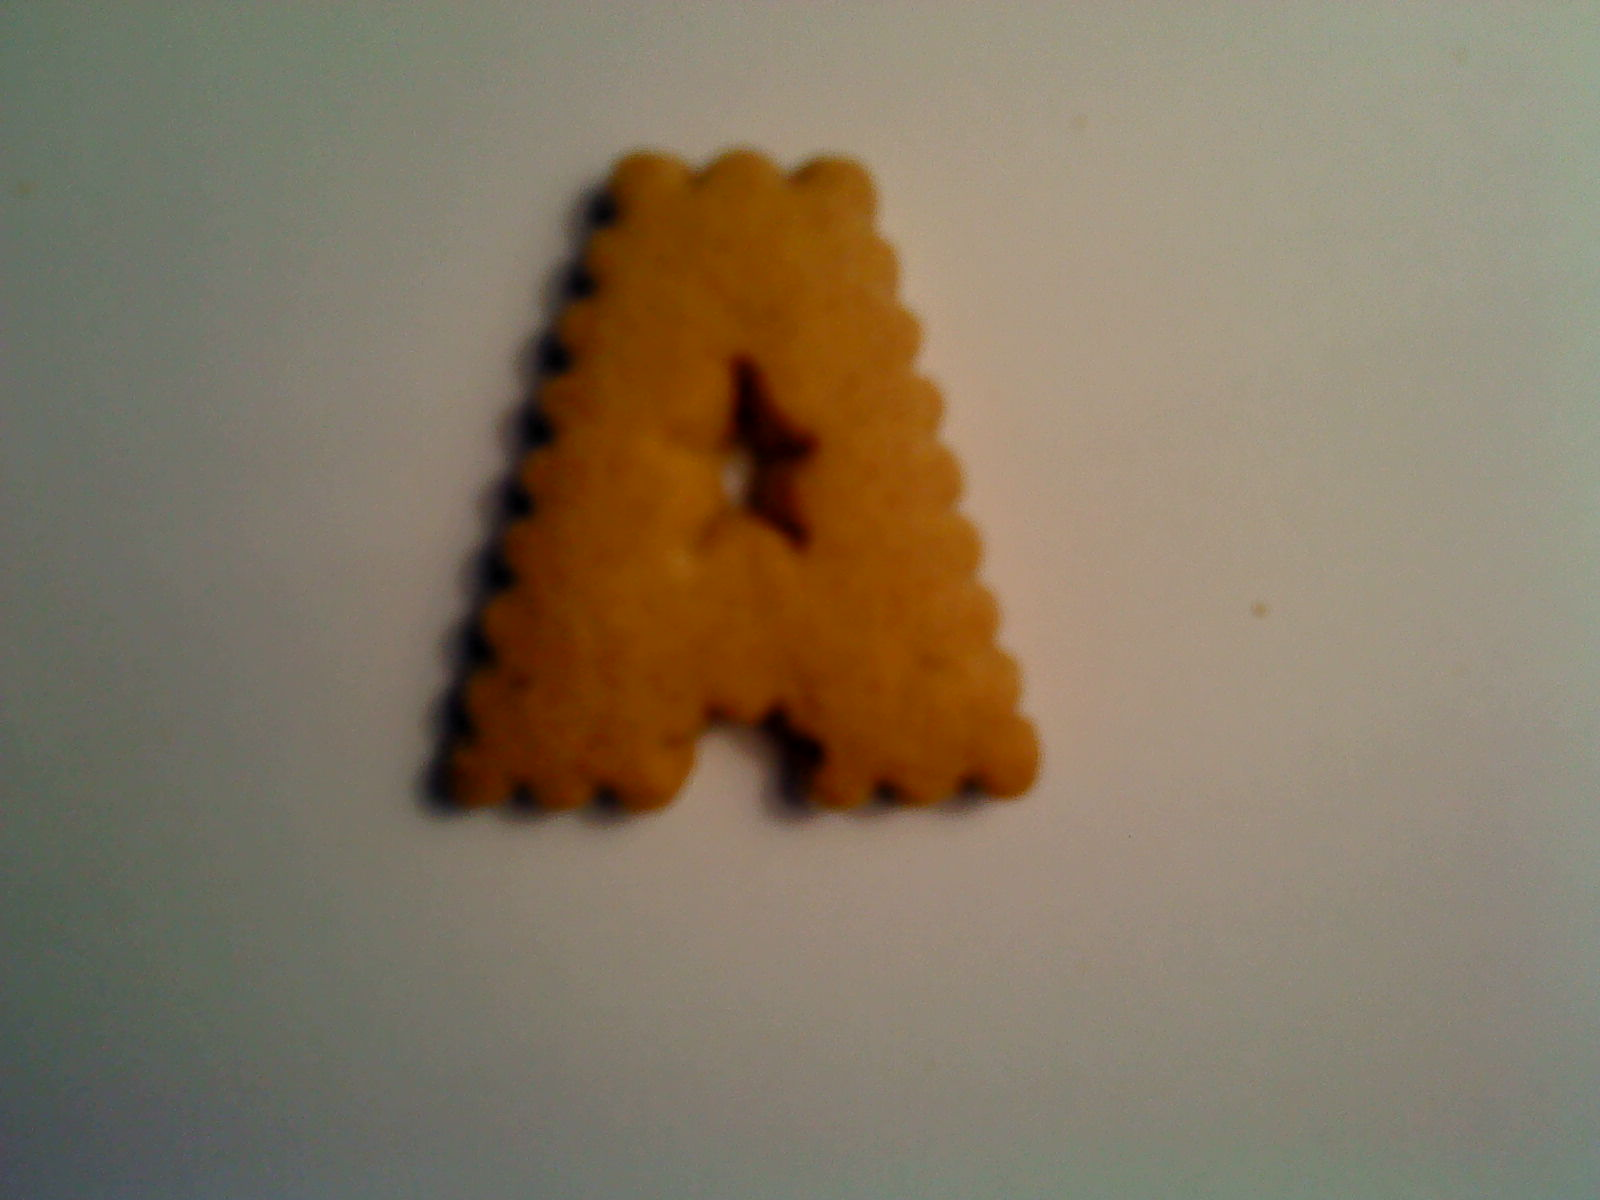
\includegraphics[width=40mm]{orig_a.JPG}
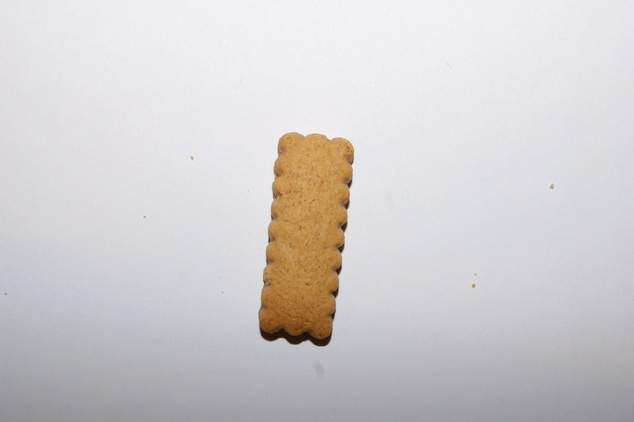
\includegraphics[width=40mm]{orig_i.JPG}
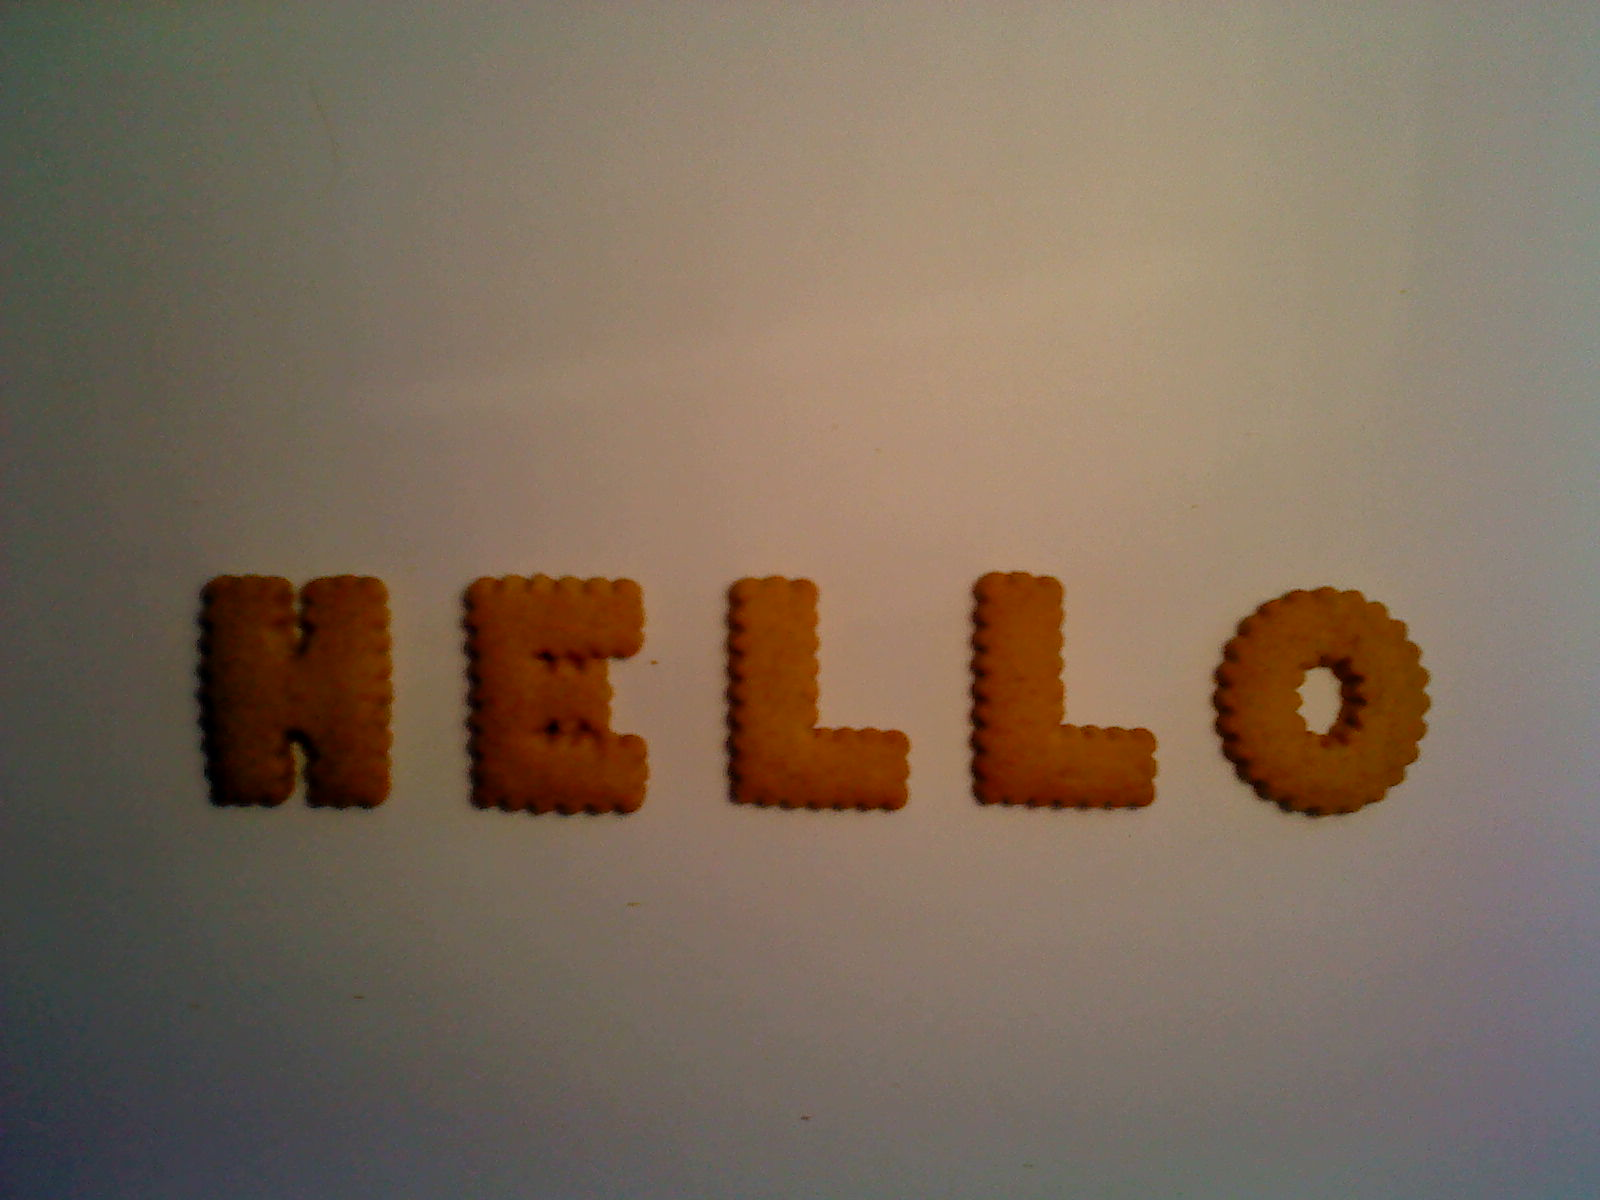
\includegraphics[width=40mm]{orig_word.JPG}
\caption{Three unprocessed images}
\end{center}
\label{fig:unprocessed}
\end{figure}

\section{Segmentation}
The segmentation is to be decided...
\section{Features}
\subsection{Feature normalization}
The features presented above are incomparable to each other.
When MajorAxisLength have been normalized with respect to the area, 
it can be compared to another MajorAxisLength value, 
even though the zooming of the pictures are not the same. 
However, the feature MajorAxisLength is incompariable to features of a different type.

In the configuration in table \ref{tab:features}, it's clear that the Solidity reveals that the biscuits
are different, the MajorAxisLength are however not to different.
However, when naively comparing by subtraction, MajorAxisLength has a bigger difference.
To battle this behavior we use the \emph{linear scaling with unit variance} normalization, see equation \ref{eqn:univariance}.
\begin{equation}
x_{new} = \frac{x-\mu}{\sigma}
\label{eqn:univariance}
\end{equation}

\begin{table}[h!b!p!]
\caption{Two features of two biscuits}
\begin{center}i
    \begin{tabular}{ l | c | c | }
                    & Biscuit 1 & Biscuit 2 \\ \hline
    MajorAxisLength & 7.0       & 8.5       \\ \hline
    Solidity        & 0.11      & 0.9       \\ \hline
    \end{tabular}
\end{center}
\label{tab:features}
\end{table}

\section{Training on known characters}
\section{Classifying unkown biscuits}
\section{Results}
\section{Discussion}
\section{References}
\section{Appendice}
\section{sec 2}

\subsection{mysubsec}
\section{Conclusions}
We got the exact result we wanted.

\end{document}
